\chapter{Introduction}
\label{ch:introduction}

\section{Problem Statement}
This project stems from the Kaggle Challenge: Evaluate Student Summaries,\footnote{\href{https://www.kaggle.com/competitions/commonlit-evaluate-student-summaries}{CommonLit - Evaluate Student Summaries - Website}} which was hosted by CommonLit. The objective of this competition was to assess the quality of summaries written by students in grades 3-12.\\
This involved developing a machine learning model to predict the scores given by human annotators for two different metrics: "Content" and "Wording", as described in \hyperref[fig:content-and-wording]{Figure~\ref{fig:content-and-wording}}.\\
\begin{figure}[h]
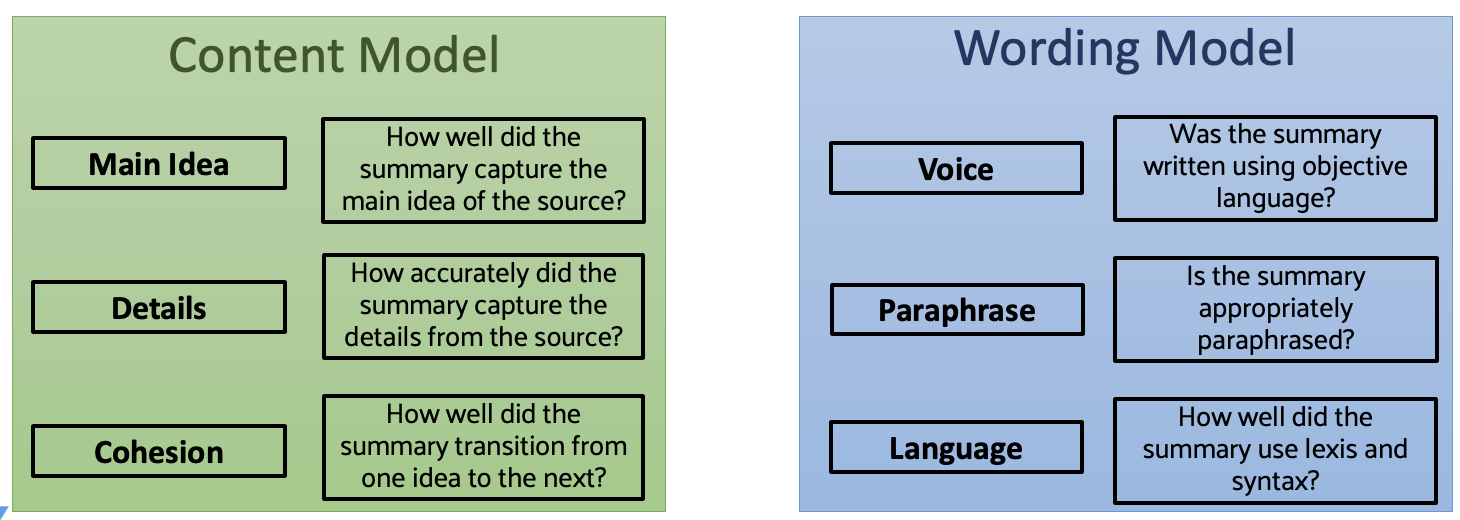
\includegraphics[keepaspectratio, width=\textwidth]{img/content_wording.png}
\caption[Description of Content and Wording]{Source: \href{https://www.kaggle.com/competitions/commonlit-evaluate-student-summaries/discussion/424402\#2349973}{CommonLit - Evaluate Student Summaries}}
\label{fig:content-and-wording}
\end{figure}\\
The human annotators were instructed to ignore grammar and spelling when evaluating the summaries. Additionally, the annotators were unaware of the students' grade levels. Meaning all summaries, regardless of what grades the students were in, were evaluated equally. This is also reflected in the data. There is no information on the students, only a unique student ID and the summary itself, together with its wording and content scores and an ID to identify to which reference text it was based on. Further details about the data are provided in \hyperref[ch:data]{Chapter~\ref{ch:data}}.

\pagebreak
\subsection{Background and Motivation of Problem}
CommonLit is a nonprofit organization dedicated to promoting reading, writing, communication, and problem-solving skills in students. Writing summaries is a crucial skill that encompasses reading comprehension, writing proficiency, and critical thinking. Unfortunately, it is a time-consuming task for teachers to read, correct, and grade students’ summaries, limiting the opportunities for students to practice these skills.\\
Being able to automatically evaluating students' writing would significantly reduce the workload for teachers. But there is a scarcity of datasets containing student writing. As a result, current techniques for summary evaluation primarily focus on automatically generated summaries rather than those created by humans, let alone students.

\section{Goal of this Work}
The primary objective of this project was to leverage the data provided by the challenge and develop a model capable of automatically predicting accurate scores. The Kaggle challenge presented two distinct prize categories: Leaderboard and Efficiency. Our focus was on the Leaderboard category, as the we believed that prioritizing accuracy over efficiency would provide a more valuable learning experience. Moreover, deliberately overfitting models was avoided, as we deemed it 
%inconsistent with the spirit of the challenge and
unrepresentative of real-world projects.

\section{Evaluation Function}
Submissions to the challenge were scored using the \gls{mcrmse}, calculated as follows:

\begin{equation}\label{eq:mcrmse}
    MCRMSE = \frac{1}{N_t} \sum_{j=1}^{N_t} \sqrt{\frac{1}{n} \sum_{i=1}^{n} (y_{ij} - \hat{y}_{ij})^2}
\end{equation}
\myequations{Mean Columnwise Root Mean Squared Error}

\noindent $N_t$ represents the number of target columns, with $N_t = 2$ in this case (one column for the content scores and one for the wording scores). The variable $n$ corresponds to the number of rows, i.e. the total number of summaries to be evaluated. And the variables $y$ and $\hat{y}$ denote the actual and predicted values, respectively.\\
In short, the \gls{mcrmse} is obtained by computing the \gls{rmse} for each of the two metrics: content and wording. The final score is then determined by averaging all the calculated \glspl{rmse} across those two metrics.\\
The range of the \gls{mcrmse} is non-negative, with 0 being the theoretical best possible score. (It can be calculated easily in Python
%\footnote{\href{https://www.python.org/}{Python - Website}}
using the scikit-learn
%\footnote{\href{https://scikit-learn.org/}{scikit-learn - Website}}
library.)
\begin{lstlisting}[language=Python]
from sklearn.metrics import mean_squared_error
rmse_content = mean_squared_error(y_true[0], y_pred[0], squared=False)
rmse_wording = mean_squared_error(y_true[1], y_pred[1], squared=False)
mcrmse = 1/2 * (rmse_content + rmse_wording)
\end{lstlisting}
